%  LaTeX support: latex@mdpi.com 
%  In case you need support, please attach all files that are necessary for compiling as well as the log file, and specify the details of your LaTeX setup (which operating system and LaTeX version / tools you are using).

% You need to save the "mdpi.cls" and "mdpi.bst" files into the same folder as this template file.

%=================================================================
\documentclass[jmse,article,submit,moreauthors,pdftex,10pt,a4paper]{mdpi} 
%
%--------------------
% Class Options:

%----------
% submit
%----------
% The class option "submit" will be changed to "accept" by the Editorial Office when the paper is accepted. This will only make changes to the frontpage (e.g. the logo of the journal will get visible), the headings, and the copyright information. Also, line numbering will be removed. Journal info and pagination for accepted papers will also be assigned by the Editorial Office.
%------------------
% moreauthors
%------------------
% If there is only one author the class option oneauthor should be used. Otherwise use the class option moreauthors.
%---------
% pdftex
%---------
% The option pdftex is for use with pdfLaTeX. If eps figure are used, remove the option pdftex and use LaTeX and dvi2pdf.

%=================================================================
\firstpage{1} 
\makeatletter 
\setcounter{page}{\@firstpage} 
\makeatother 
\articlenumber{x}
\doinum{10.3390/------}
\pubvolume{xx}
\pubyear{2017}
\copyrightyear{2017}
\externaleditor{Academic Editor: name}
\history{Received: date; Accepted: date; Published: date}

%------------------------------------------------------------------
% The following line should be uncommented if the LaTeX file is uploaded to arXiv.org
%\pdfoutput=1

%=================================================================
% Add packages and commands here. The following packages are loaded in our class file: fontenc, calc, indentfirst, fancyhdr, graphicx, lastpage, ifthen, lineno, float, amsmath, setspace, enumitem, mathpazo, booktabs, titlesec, etoolbox, amsthm, hyphenat, natbib, hyperref, footmisc, geometry, caption, url, mdframed, tabto, soul, multirow, microtype
\usepackage{subcaption}

%=================================================================
% Full title of the paper (Capitalized)
\Title{Sea Level Forecasts Aggregated from Established Operational Systems}

% Authors, for the paper (add full first names)
\Author{Andy Taylor $^{1}$, Gary B Brassington $^{1}$ and Someone Else $^{2,\ddagger}$*}

% Authors, for metadata in PDF
\AuthorNames{Andy Taylor, Gary Brassington}

% Affiliations / Addresses (Add [1] after \address if there is only one affiliation.)
\address{
$^{1}$ \quad Bureau of Meteorology; 700 Collins St Docklands 3008, Australia} 

% Contact information of the corresponding author
\corres{Correspondence: Andy.Taylor@bom.gov.au; Tel.: +61-3-9669-4650}

% Current address and/or shared authorship
%\firstnote{Current address: Affiliation 3} 
%\secondnote{These authors contributed equally to this work.}
% The commands \thirdnote{} till \eighthnote{} are available for further notes

% Simple summary
%\simplesumm{}

% Abstract (Do not use inserted blank lines, i.e. \\) 
\abstract{ A system for providing routine 7-day forecasts of sea level observable at tide gauge locations is described and evaluated.
Forecast timeseries are aggregated from well established operational systems of the Australian Bureau of Meteorology operations; though these systems are only quasi-complimentray.
The forecasts can add value to routine coastal decision processes under non-extreme conditions; such as seagate and fish weir operations, under keel clearance systems and flood warning models. Practical levels of skill are demonstrated for such applications at a range of locations in the Australian region.
The configuration is relatively robust to operational realities such as version upgrades, data gaps and metadata ambiguities.
Forecast skill is evaluated against hourly sea level observations at tide gauge locations.  Notable exceptions to application include extreme forcing scenarios such as tropical cyclones, tsunami.
Characteristics of the bias correction term are demonstrated to be primarily static in time, but with time varying signals showing some spatial coherence.
Concluded that the current simple configuration provides limited but potentially useful levels of skill.; and that interpolation between observations sites could be meaningfully pursued. Furthermore, this general aggregation approach may prove to be optimal for routine sea level forecast services given the phyically inhomogeneous processes involved.}
           
% Keywordsi
\keyword{forecasting; sea level; tides; Australia, operational oceanography}


%%%%%%%%%%%%%%%%%%%%%%%%%%%%%%%%%%%%%%%%%%
% Only for the journal Data:
%\dataset{DOI number or link to the deposited data set in cases where the data set is published or set to be published separately. If the data set is submitted and will be published as a supplement to this paper in the journal Data, this field will be filled by the editors of the journal. In this case, please make sure to submit the data set as a supplement when entering your manuscript into our manuscript editorial system.}
%\datasetlicense{license under which the data set is made available (CC0, CC-BY, CC-BY-SA, CC-BY-NC, etc.)}

%%%%%%%%%%%%%%%%%%%%%%%%%%%%%%%%%%%%%%%%%%
% For Conference Proceedings Papers: add the conference title here
%\conferencetitle{}
%\setcounter{secnumdepth}{4}
%%%%%%%%%%%%%%%%%%%%%%%%%%%%%%%%%%%%%%%%%%

\begin{document}

%%%%%%%%%%%%%%%%%%%%%%%%%%%%%%%%%%%%%%%%%%
% \setcounter{section}{-1} %% Remove this when starting to work on the template.
%\section{How to Use this Template}
% The template details the sections that can be used in a manuscript.
%Note that the order of %article sections may differ from the requirements of the journal
%(e.g. for the positioning of the Materials and Methods section).
%Please check the instructions for authors page of the journal to verify the correct order.
%For any questions, please contact the editorial office of the journal or support@mdpi.com.
%For LaTeX related questions please contact Janine Daum at latex-support@mdpi.com.

%%%%%%%%%%%%%%%%%%%%%%%%%%%%%%%%%%%%%%%%%%
\section{Introduction}

\subsection{Context}

% still sea level is relevant
Of the activities that now constitute 'operational oceanography' \cite{Bell:2009uv}, sea level forecasting possibly has the most historical baggage as well as the most widespread application.
Day-to-day routine decisions are based on expectations of still water level \cite{Pugh:2014vf} at the coast.  
For example in sea-gate and fish weir operations [REF], under keel clearance systems [REF], coastal works scheduling and indirectly for activities at river mouthes (ee QLD dam outflow) [REF] 
Extreme variations in sea level, such as due to tropical cyclones and tsunami, are not the focus of the present document.


\subsection{operational and practical}
All models are wrong, some are useful ...and some are operational.\\

% evolution of targeted physical models
% ...tides, surge, circulation, waves, 

practical importance of 'operational' status
 ...cultural embeddedness 
...newness in operations -> trust, risk and sustainment\\

Data driven versus dynamics ...
complete generalised model are increasingly realistic\\
% ... but typically a comprimise/trade-off 
% ... role of DA 
% 

\subsection{different physical contributions}
 ...mix, regional balance




% plenty of downscale and 


% contributors
Sea level contibuting factors.\\
Diverse processes -> evolution of specialised modelling approaches for different time scales and processes\\
Many routine decisions dont care about distinctions ...just need to know the sea level.\\
Nested downscaling offers many attractions but may not prove to be the optimal approach for services.  Futhermore, nesting approaches have been motivated by technological limitations rather than phyicss .... contract adapative meshes, tidal ephemeris etc\\

Australia is a large domain tha highlights varianble balance of processes.\\


\subsection{tide predictions as special class of data driven}

Conventional tide predictions are a remarkaby successful forecast product that provide an omni-present reference for coastal activities.
By design these unique predictions make no account for the aperiodic phemomena that constitute 'non tidal' energy. 
Production involves timeseries statistics based on historical records of observations at each forecast site.
Tidal techniques exploit the significance of periodic sea level variations observed to be coherent with the astronomical tide producing forces (ATGF) \cite{Hendershott:1981ub}.     
By assuming that historical coherence is time invarient, astronomical motions can be mapped to predicted sea level via an admittance function.   
Useful sea level predictions can thereby be produced many years into the future.  
Many variations exist for implementing this general approach (eg \cite{Foreman:2009bg}, \cite{Groves:1975ky},\cite{LEFFLER:2009ej},\cite{Smith:1997ut} ). 
But tidal methods based on a harmonic decompostion of the ATGF have long been typical of bodies promolgating 'official' tidal products; including the Australian Bureau of Meteorology.
Statistical properties of offical tidal predictions have come to define elevation references for mapping and legal applications \cite{PCTMSL:2009vy}.
%In Australia tidal activities are distributed between the Bureau of Meteorology and the Australian Hydrographic Service (now a section of Geospatial Intellegence Unit of Defence).


% periodic but not astro 
The ongoing value of standard tidal predictions reflects the fact that periodic signals generally dominate coastal still water levels.
It is notable however that the physical drivers of sea level represented in tidal predictions need not be graviational at all; for instance at longer periods \cite{Parker:2007wq}
The extent to which conventional harmonic tidal predictions are 'physics free' actually allows for a pragmatic flexibilty to represent almost all of the everyday rise and fall of coastal sea level at a place.
Purely physical models of ocean tides are really only of academic interest (eg \cite{Weis:2008ex} \cite{Muller:2008hs}).
Important spatial tidal solutions ultimately draw a trade-off between physics and observations \cite{Egbert:1996vr}; that is, gridded tidal products are inferior to a standard tide.



\subsection{real time obs}
 reality
 QA
 
 
\subsection{dynamic models and DA}

% downscaling and models
In contrast to the 
Application of primative equation dynamic models to the task of forecasting routine coastal sea level is increasingly relevant,  to reto provide operational 
There has been much scientifc  canonical approach to coastal forecasting in the operational oceanographic context is via dynamical downscaling eg \cite{Paramygin:2017dx} \cite{Garzon:2016ds}.
Regional dynamic downscaling of OceanMAPS forecasts is undertaken by the Bureau for special applications (cites?),
but spatial and temporal coverage is not yet comprehensive.\\
Dedicated storm surge forecasting systems have been developed and are currently in transition to operational support (cite Greenslade CandP).   These new systems are based on higher resolution barotropic-only models, without no outer nesting global model, over shorter forecast windows. These new surge forecast systems are not addressed further in this document. \\


More

The capability of the Australian Bureau of Meteorology (BoM) to operationally observe and forecast the ocean has expanded in the last decade;
and recent efforts are increasingly directing towards coastal regions.  
It is notable that operationally supported systems are designed and configured in a manner distinct from academic modelling studies. 
Several existing operationally supported systems involve aspects of coastal sea level;
but these are only quasi-complimentary with regard to providing practical sea level forecasts over synoptic timescales. \\


What is available now?\\
Exlusion of wave setup - parsimony and typically out of surf zone.\\
Riverine inputs ...not included though aggSL is feed into dependant ratings \\


A diverse range of 'users' make decisions that involve expectations about sea level. 
But the academic decomposition of signals attributed to observed sea level is often irrelevant or a source of miscommunication. 

Forecasts need to be fit-for-purpose and reliably available: all models are wrong, but some are useful \cite{Box:1979hl} .

The Australian coastline spans a vast geographic extent that features long regions of interconnected oceanography \cite{Ridgway:2004kb}, \cite{Church:1986tl}, \cite{Haigh:2013bn}, \cite{Woodham:2013cl}.  Across this domain the balance of physical contributions to coastal sea level variation is diverse.\\


Bureau operations include conventional harmonic analysis and tide tables.
These continue to provide a foundational and unique forecast product with myriad applications.
Although harmonic analysis is based on historical records, real-time communication of tide gauge observations has become the norm.
The Bureau operates its own network of tide gauges \cite{Greenslade:2012um} but also ingests observations from many operated by partner organisations.   
Gathering observations from diverse organisations is valuable but can raise issues with data qualuity and metadata managment.



'Operational oceanography' \cite{Bell:2009uv} has matured in a manner analogous to numerical weather prediction (NWP).
Near-global ocean forecasts have been in operational production now for 10 years via several versions of OceanMAPS  
\cite{Brassington:2007ut}\cite{NMOC:2007wq}\cite{BureauofMeterology:2011ta}\cite{Brassington:2012wm}.
The current version of this data-assimilating primitive equation forecast system is configured to represent mesoscale ocean variability with regular structured horizontal discretisation of 0.1x0.1 degrees.
Forecasts for the next 7-days are produced daily using a multi-cycle ensemble schedule \cite{GaryBBrassington:2013jw}.



%The introduction should briefly place the study in a broad context and highlight why it is important.
%It should define the purpose of the work and its significance.
%The current state of the research field should be reviewed carefully and key publications cited.
%Please highlight controversial and diverging hypotheses when necessary.
%Finally, briefly mention the main aim of the work and highlight the principal conclusions.
%As far as possible, please keep the introduction comprehensible to scientists outside your particular field of research.
%Citing a journal paper \cite{ref-journal}. And now citing a book reference \cite{ref-book}.
%Please use the command \citep{ref-journal} for the following MDPI journals,
%   which use author-date citation: Arts, Econometrics, Economies, Genealogy, Humanities, IJFS, JRFM, Laws, Religions, Risks, Social Sciences.


%%%%%%%%%%%%%%%%%%%%%%%%%%%%%%%%%%%%%%%%%%
\section{Forecast System Concept}

The concept is a simple but careful linear superposition to provide an enhance tide prediction.
Heterogeneous operational sea level systems are aggregated into a single package to better exploit existing information.
Particularly so as to facilitate direct comparison to recent observations.

Systems to include/exclude:\\


\subsection{Motivation}
This approach is motivated by the immediate potential of exploiting existing systems to present useful sea level guidance;  7-day forecasts that can be directly evaluated against tide gauge observations.
A secondary motivation is to establish a performance benchmark against which new sea level forecast capabilities can be evaluated. \\

%\subsection{Hypothesis}
%\begin{itemize}[leftmargin=*,labelsep=5.8mm]
%\item Value is timesscale dependant: relatable to length scales in ocean model
%\item forecast skill decays with lead time
%\item Dynamic models add forecast value beyond persistence only beyond ?
%\item Ocean model adds information beyond that available in local wind forecast.
%\item Bias correction accounts for (1) fixed offsets (2) inadequately resolved physical %phenomena of large spatial scale.
%\end{itemize}
 


% hthe represent relative timing of contributing phenomena;
The concept is schematically illustrated in Figure \ref{fig:aggSL} and elements are detailed in subsequent sections.  

\begin{figure}[H]
\centering
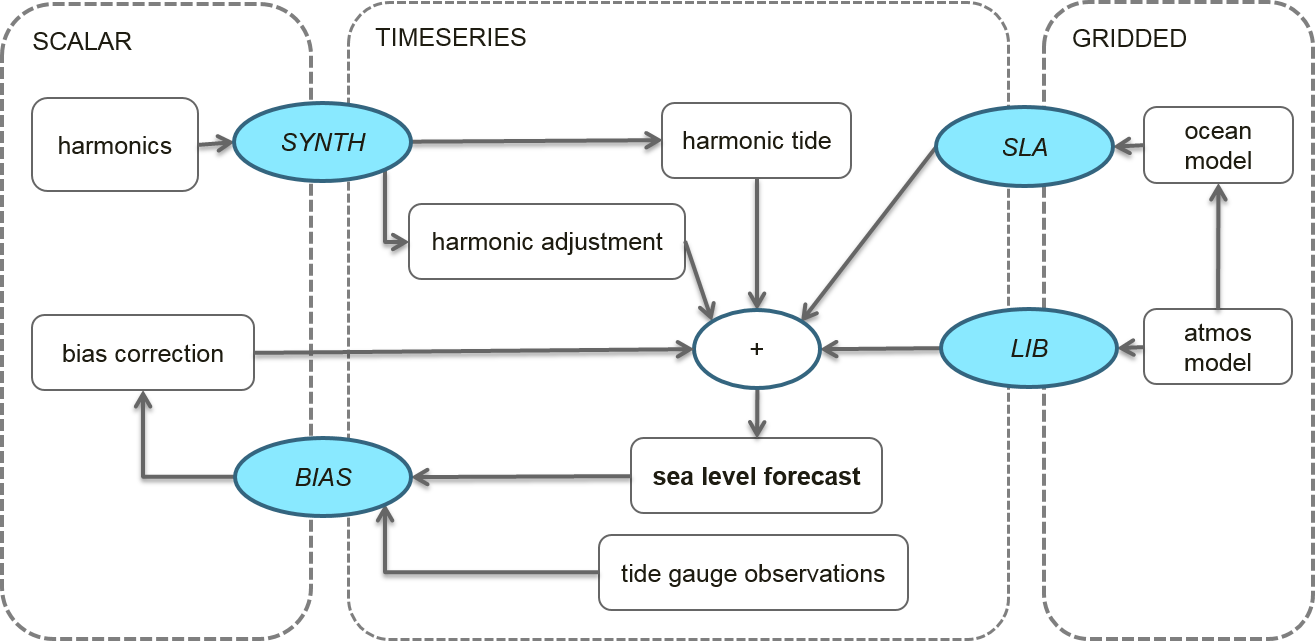
\includegraphics[width=15 cm]{plots/aggSL_schematic_abstract.png}
\caption{Schematic illustration of aggregation (\textbf{SYNTH}) etc. }
\label{fig:aggSL}
\end{figure}   




%\caption{This is a figure, Schemes follow the same formatting. If there are multiple panels, they should be listed as: (\textbf{a}) Description of what is contained in the first panel. (\textbf{b}) Description of what is contained in the second panel. Figures should be placed in the main text near to the first timcan.e they are cited. A caption on a single line should be centered.}


\subsubsection{Dynamic primitive equation models}

NWP\\
OceanMAPS\\

Noted the DA inputs and spatial coverage.\\
Altimeters cut off at 200m bathy ...because of corrections.



\begin{figure}[H]
    \centering
    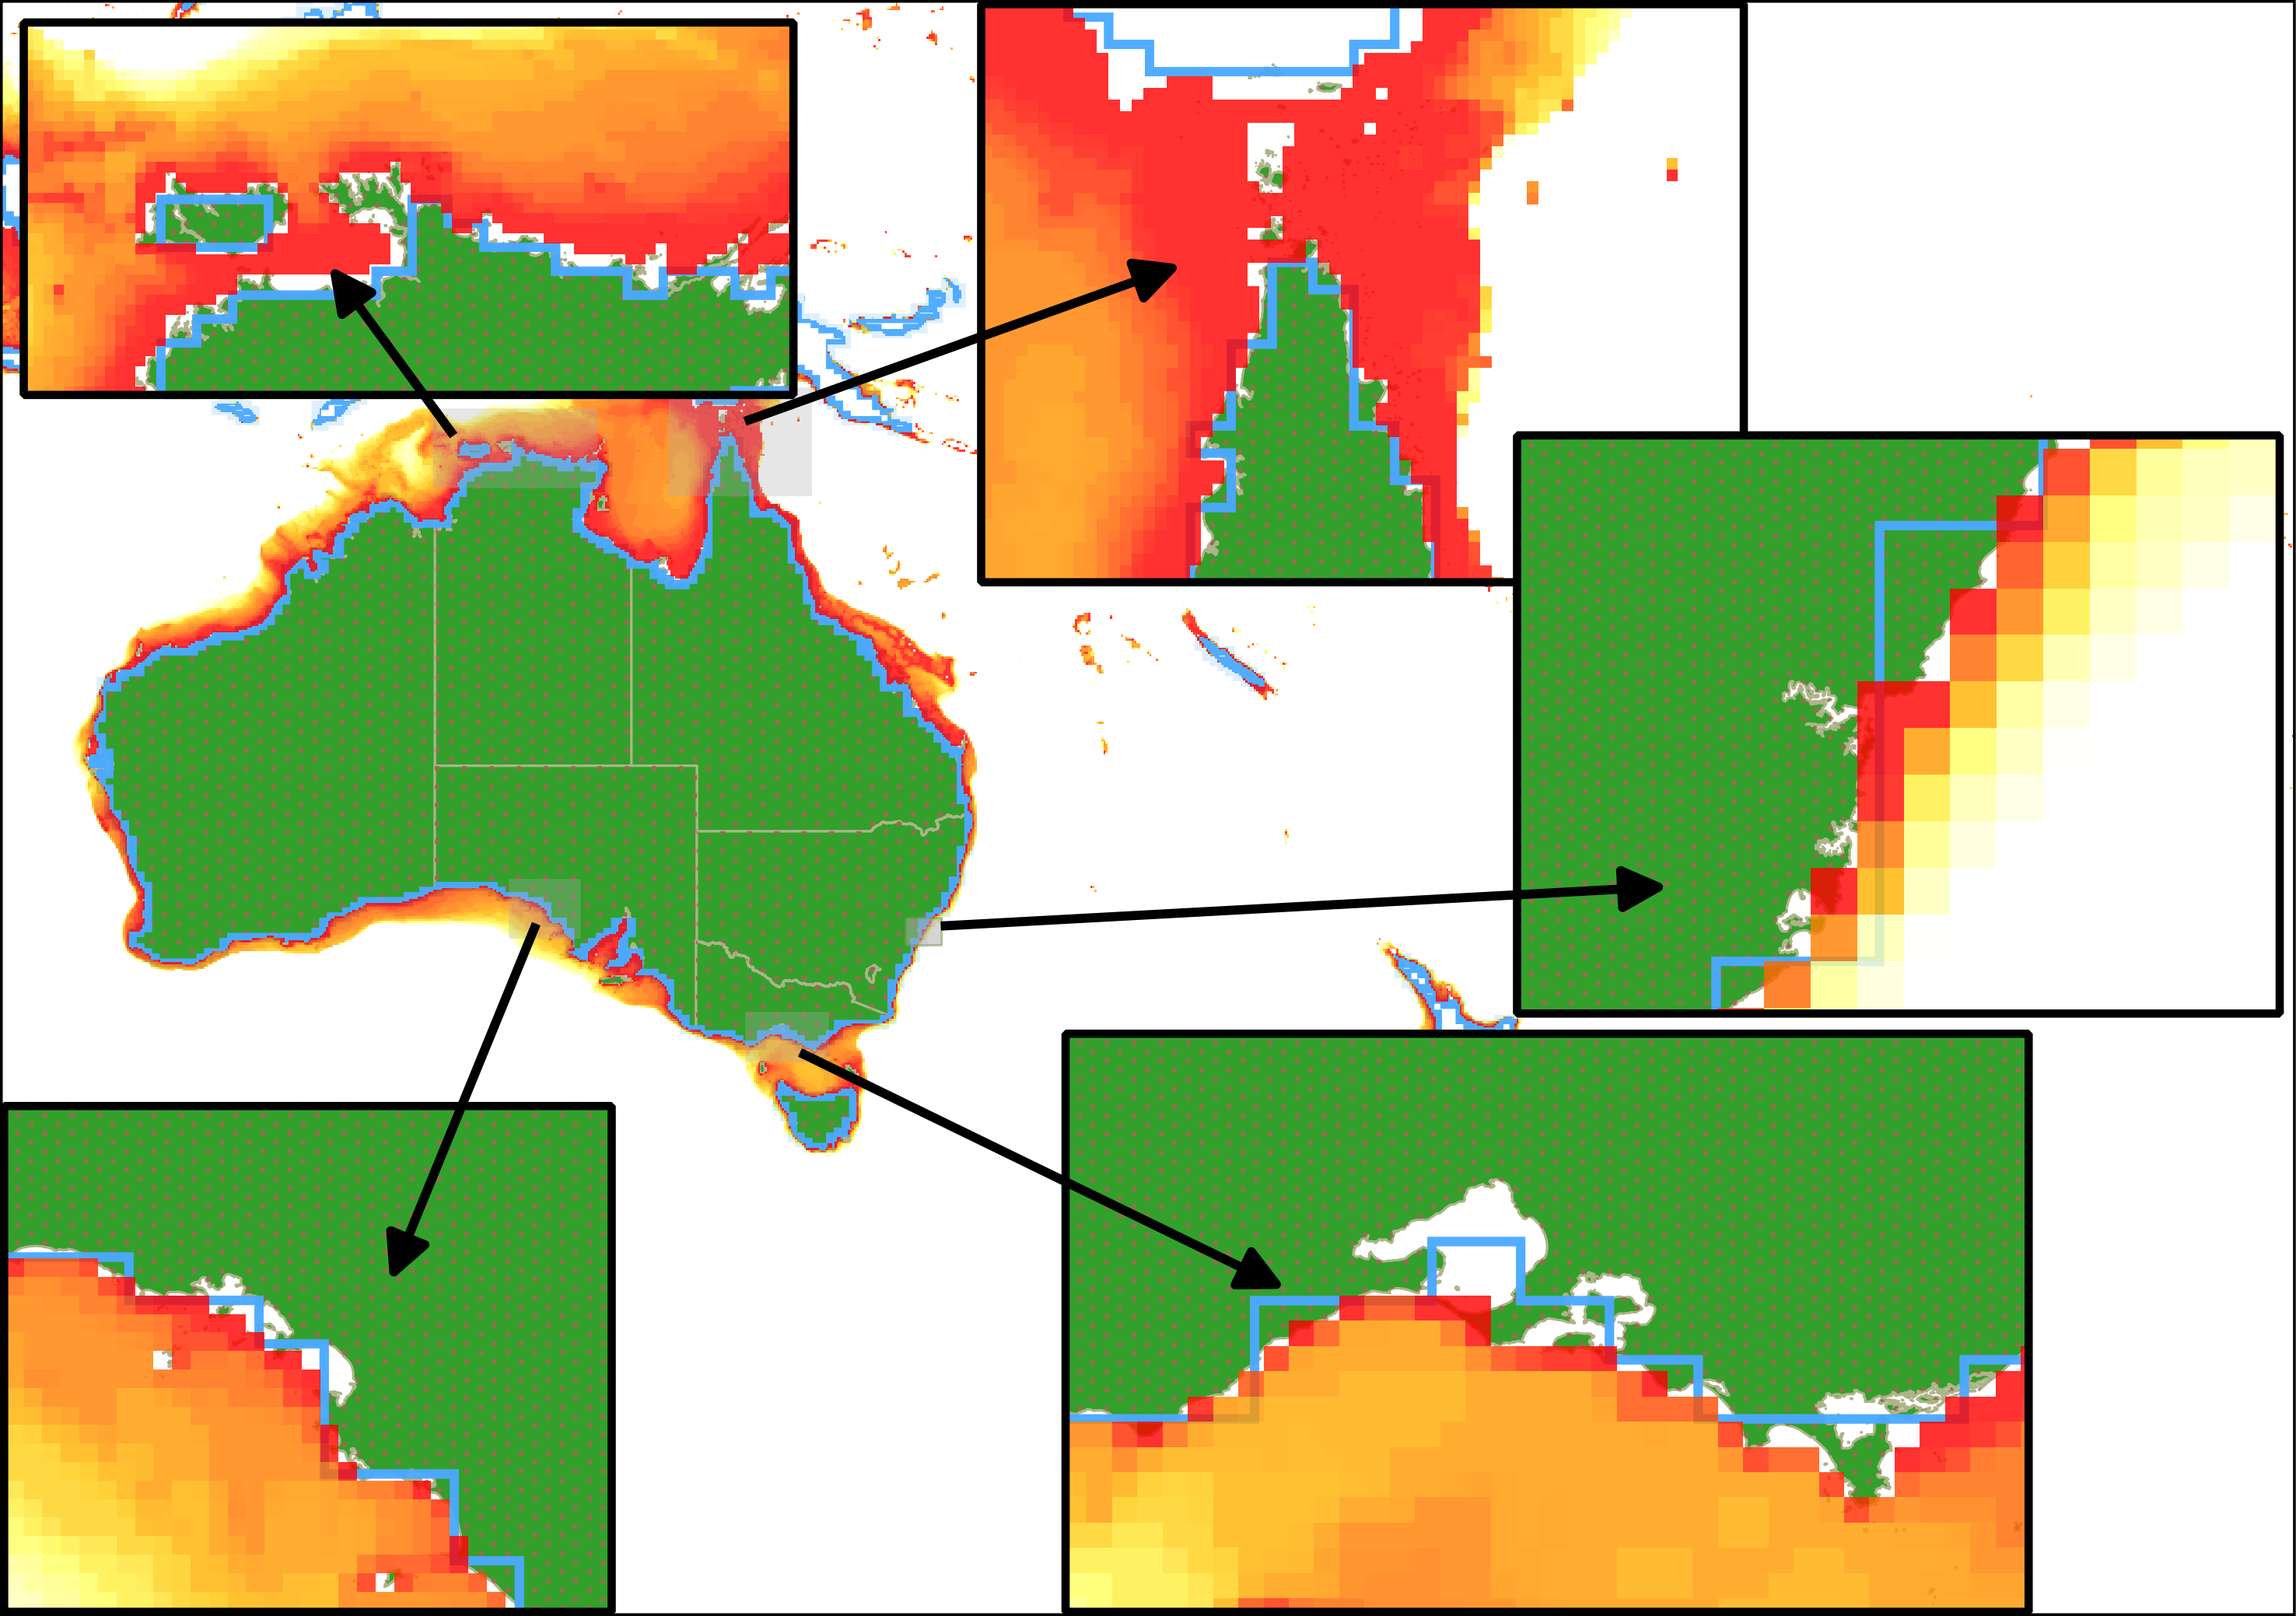
\includegraphics[width=1.0\textwidth]{plots/omaps_masks.png}
    \caption{Illustration of coastline representation. Two 'masks' are show; (1) the ocean model coastal bathymetry shown as blue squares (2) edge of atmospheric model land/sea mask shown as orange line.   Most small scale features and embayments are only approximately represented at best }
    \label{fig:map_masks}
\end{figure}  

Free surface ($\eta$).\\
Comments on non-tidal, hyrdostatic ...timescales\\


Local inverse barometer approximation:\\
why LIB?\\
reference pressure.




\subsubsection{Harmonics}
Motivation to align with Bureaus own official tide predictions.\\
Synthesize timeseries using common harmonic analysis results and software\\

Spectral overlap:\\
Harmonic analysis for standard tide tables aims to respresent total sea level (as distinct from identifying gravitation component of sea level).\\
Pragamatic approach\\
Identify apriori list of harmonics expected to be primarily non-gravitational in origin ...and thus likely to be better represented by dynamic contibution from OGM and NWP pressure.\\
'Harmonic  adjustment'.




\subsubsection{Bias correction}
Motivation:\\
Baysian idea of making best guess given available information\\
Generic aplpication (no training required)\\
Elucidate origin of mismatches.


Apriori config choices:\\
weighted causal filter (no 'future' influence)\\
Timescale 
 

Temporal evolution explored in section XX below..
  

%Bulleted lists look like this:
%\begin{itemize}[leftmargin=*,labelsep=5.8mm]
%\item	First bullet
%\item	Second bullet
%\item	Third bullet
%\end{itemize}

%Numbered lists can be added as follows:
%\begin{enumerate}[leftmargin=*,labelsep=4.9mm]
%\item	First item 
%\item	Second item
%\item	Third item
%\end{enumerate}

\subsubsection{Geographic overview}

Global\\
Focus here on Australia region.


\begin{figure}[H]
    \centering
    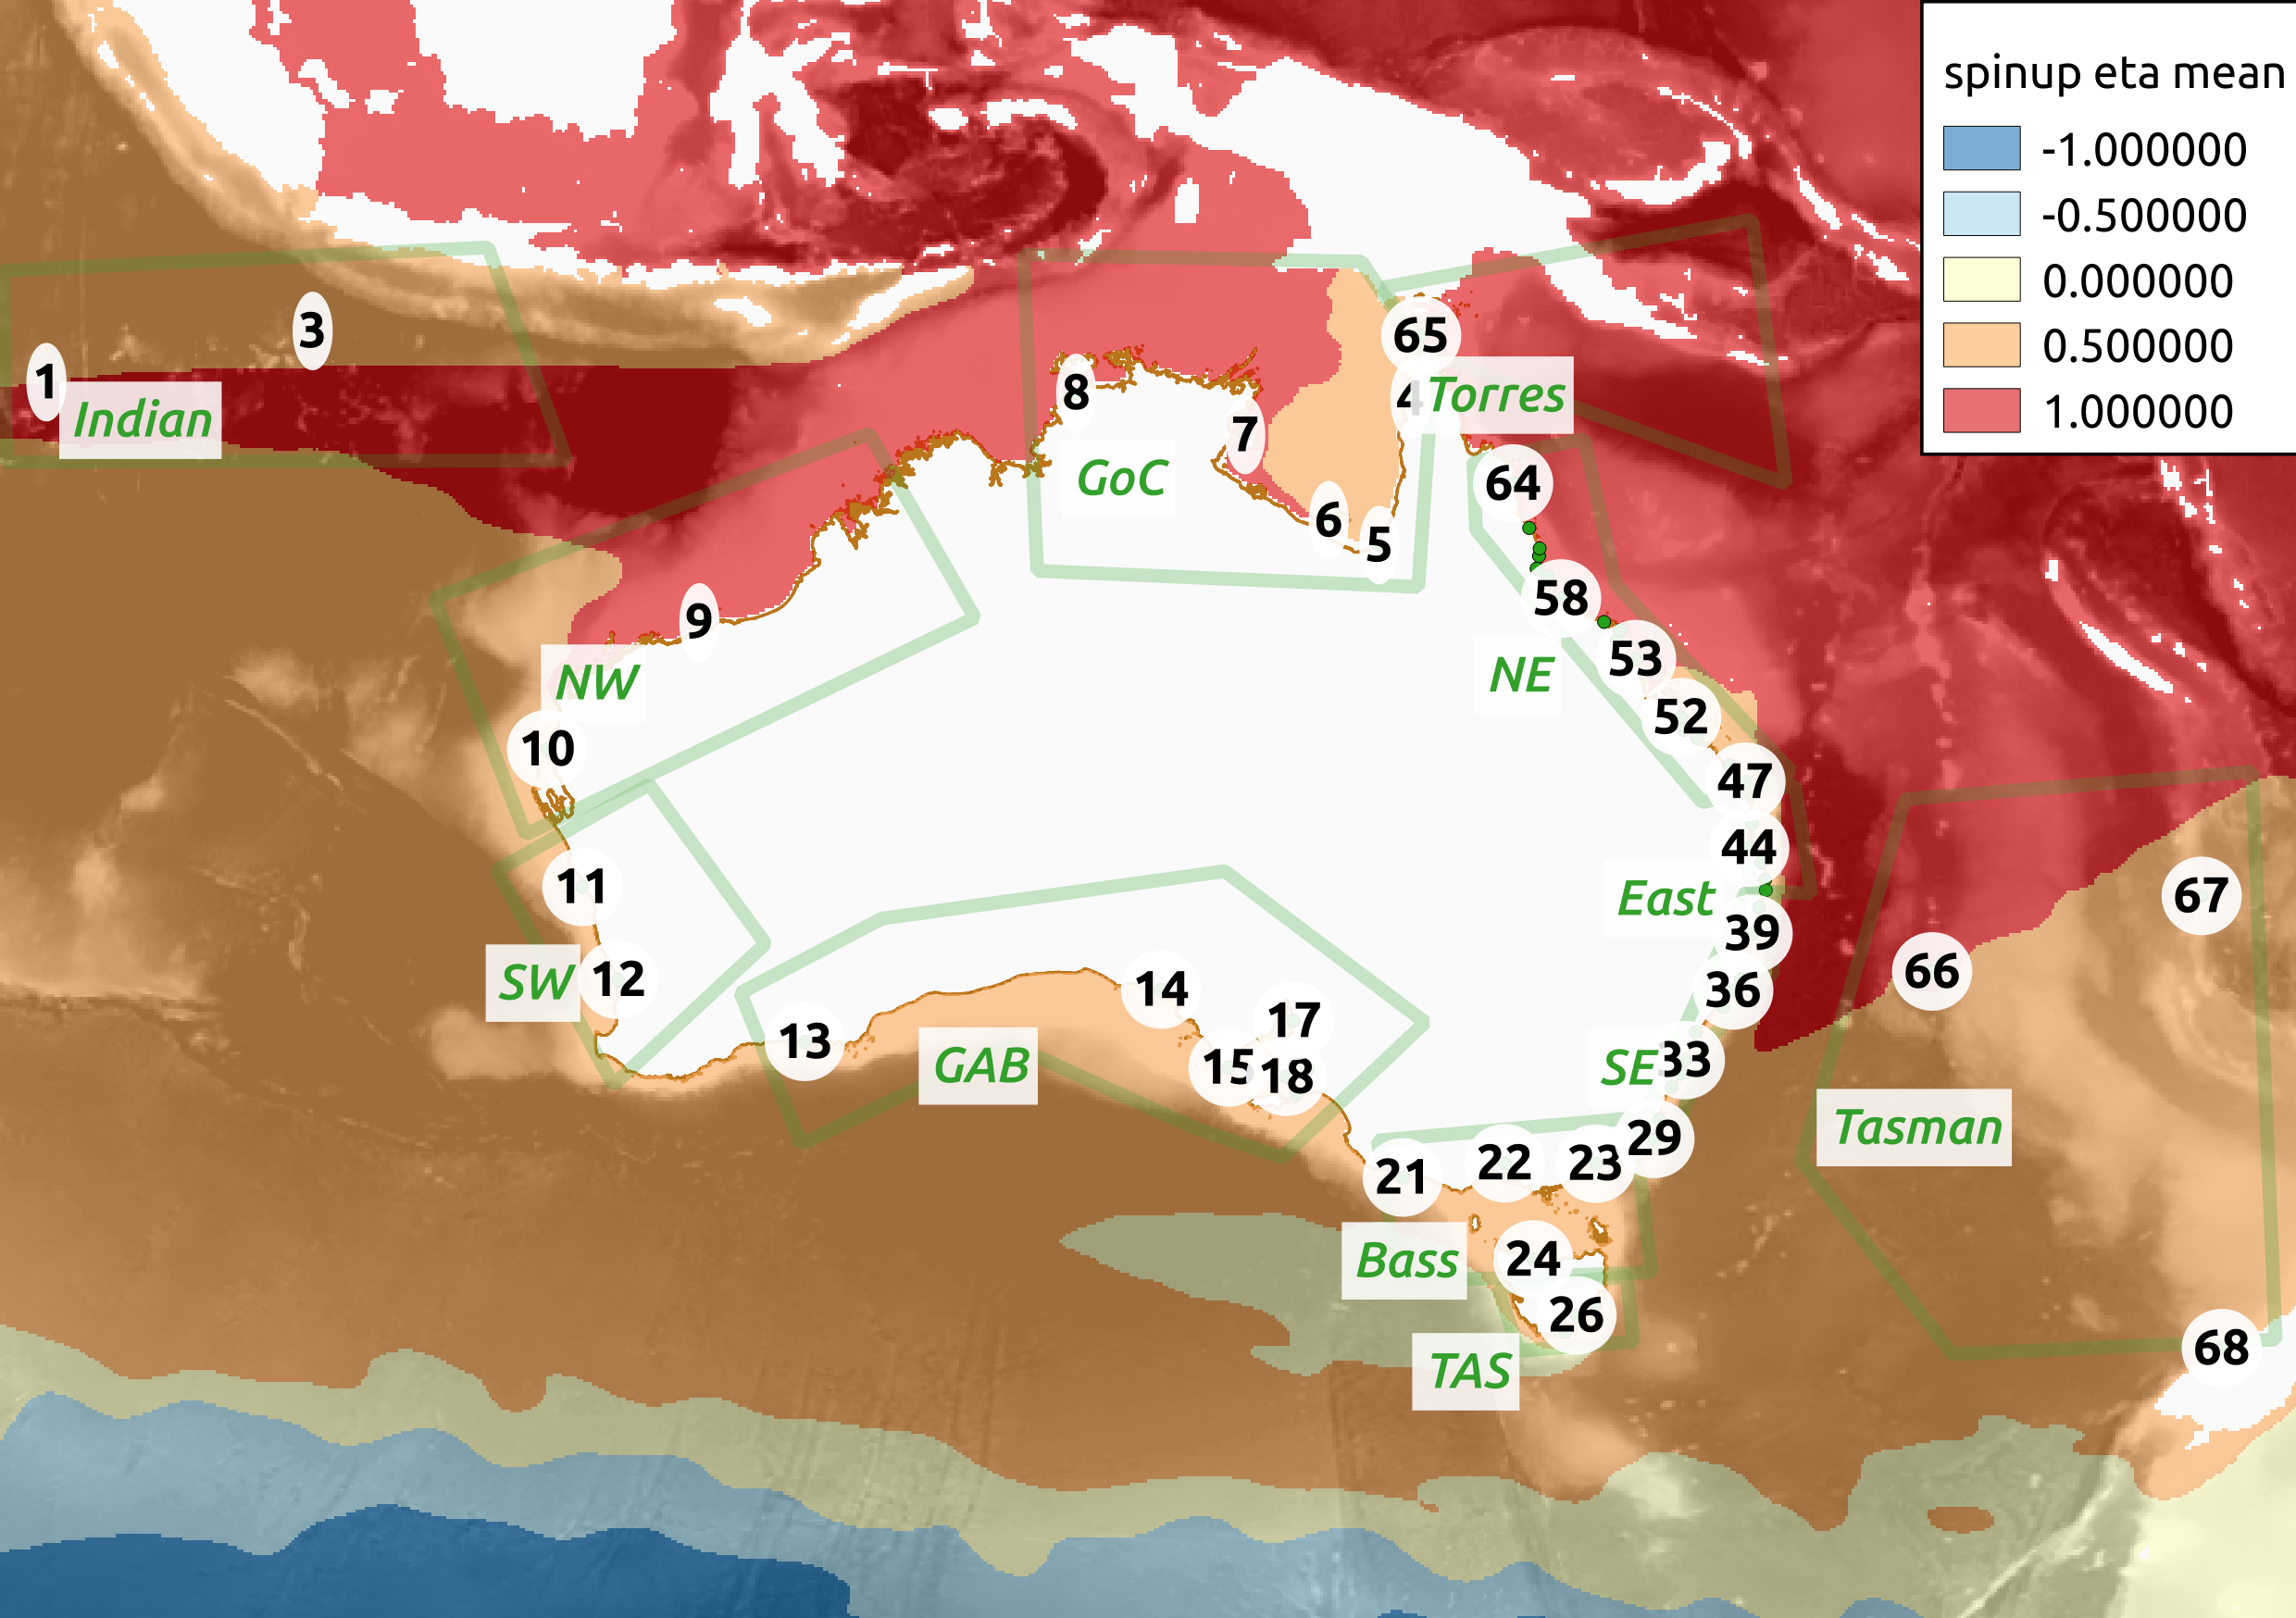
\includegraphics[width=1.0\textwidth]{plots/omaps_bathy_and_eta.png}
    \caption{Geographic overview of Australia region.  Ocean model bathymetery is indicated by grey background shading.  Colour contours illustrate the 'spinup' model mean dynamic topography referenced below.  Tide gauge locations are identified with sequential numbers with order chosen to laregly align with Kelvin wave progagation direction. Regional groupings are referenced in subsequent results.}
    \label{fig:map_locations}
\end{figure}  


%%%%%%%%%%%%%%%%%%%%%%%%%%%%%%%%%%%%%%%%%%
\section{Evaluation}


Version and operational data set.\\
Inclusion/exclusion.


\subsection{Forecast Goodness}

REF to murphy\\
Quality and Value.\\
Marginal value?? ...ie any better than existing?.\\



\subsection{Application as routine general guidance}

What is relevant ?
Tide\\
Tide +persisted residual\\

Noted - excluding categorical and event focus.



\subsection{Illustration varying skill and mix}.

%   \begin{figure}[H]
%       \centering
%       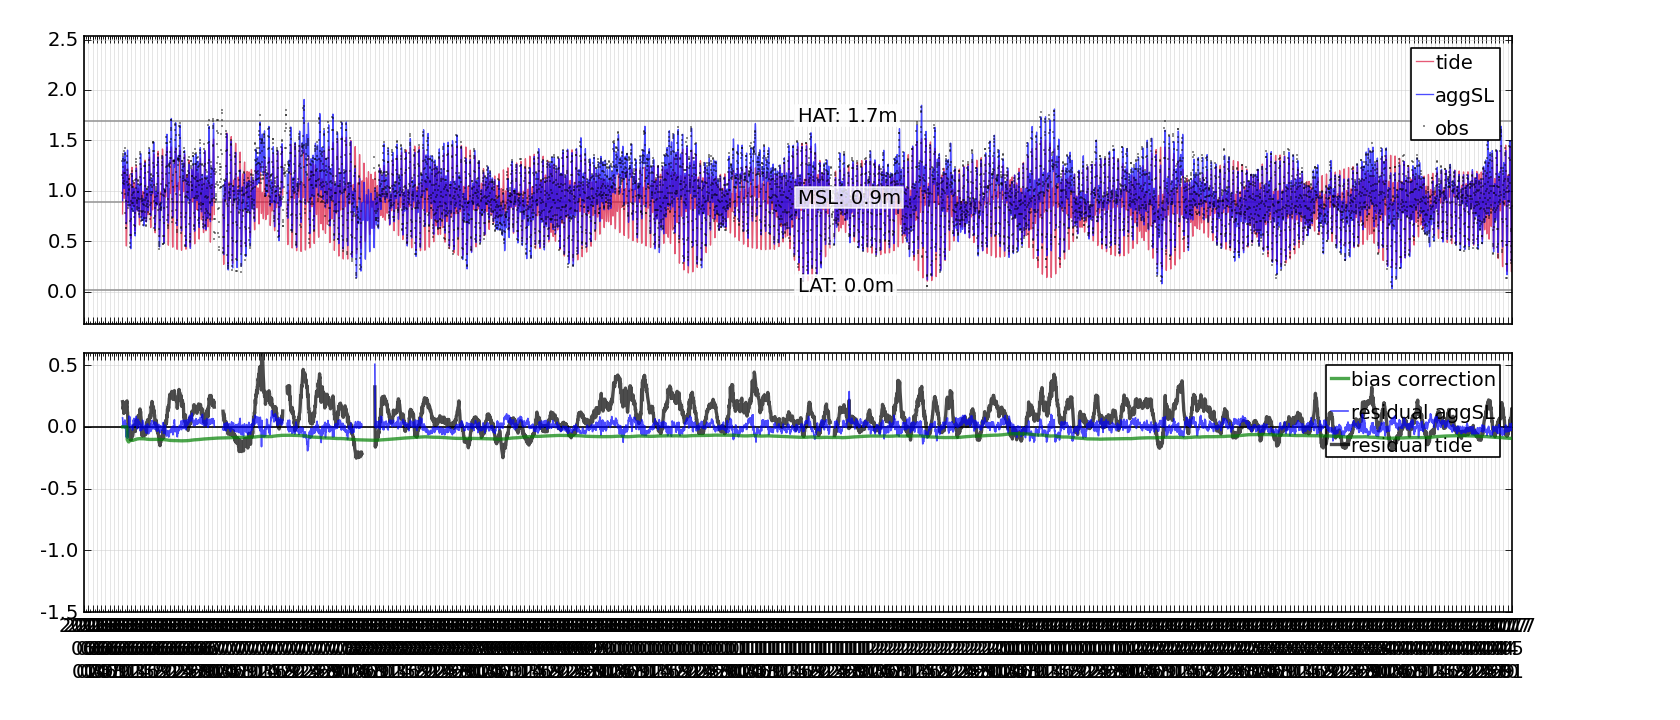
\includegraphics[width=\textwidth]{plots/0026_plot_timeseries.png}
%       \caption{ Example timeseries record for location at Melbournecp  (\textbf{23 in Figure \ref{fig:map_locations}} ); Reduction in error variance relative to harmonic tides reflects influence of sea level phenomena of greater spatial scale than local embayment}
%   \end{figure}   


\begin{figure}[H]
\centering
    \begin{subfigure}[b]{0.3\textwidth}
        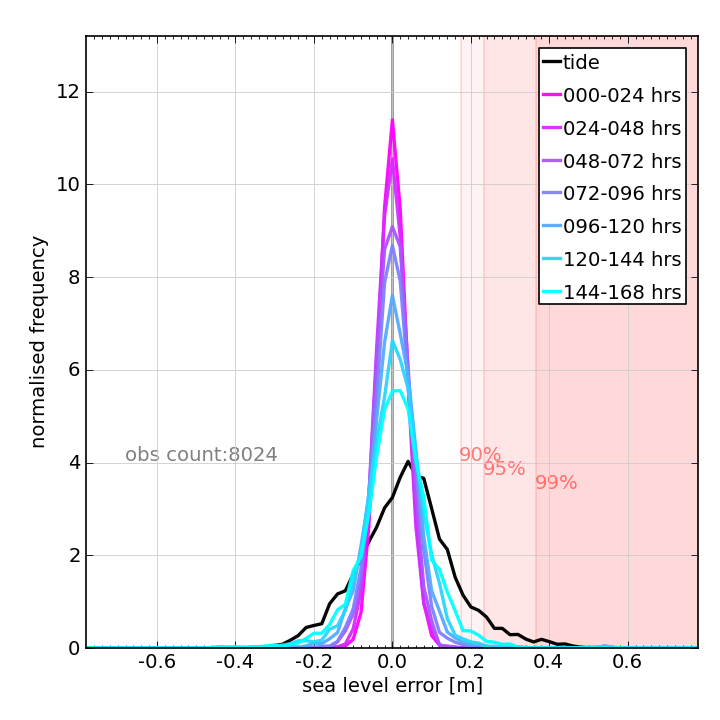
\includegraphics[width=\textwidth]{plots/0013_verify_pdf.png}
        \caption{Midlatitude storms}
    \end{subfigure}
    \begin{subfigure}[b]{0.3\textwidth}
        \includegraphics[width=\textwidth]{plots/0046_verify_pdf.png}
        \caption{tide prediction datum}
    \end{subfigure}
        \begin{subfigure}[b]{0.3\textwidth}
        \includegraphics[width=\textwidth]{plots/0006_verify_pdf.png}
        \caption{long period}
    \end{subfigure}
\caption{ Relative error metrics at selected locations. Skill gain relative to persisted residuals is only apparent in locations where synoptic scale dynamics are dominant}
\label{fig:pdf_c}
\end{figure}   


\begin{figure}[H]
\centering
    \begin{subfigure}[b]{0.3\textwidth}
        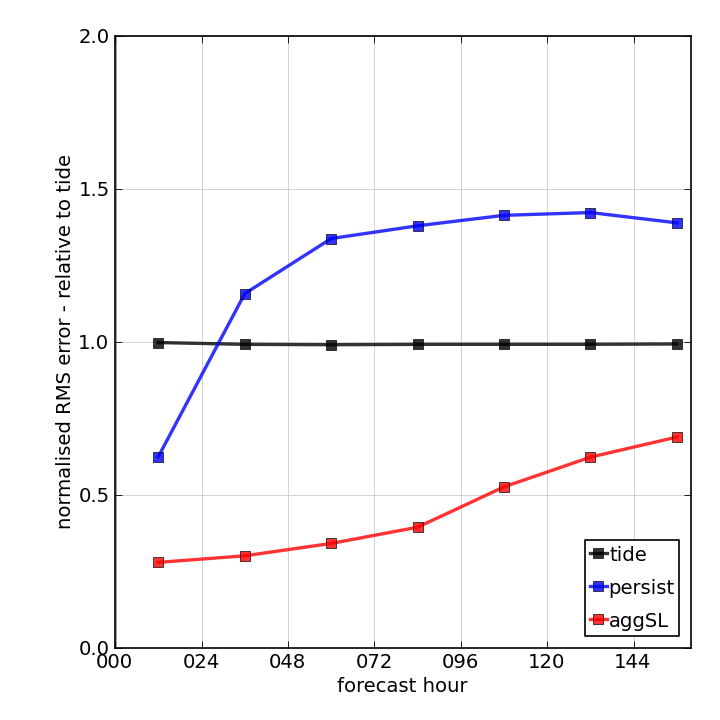
\includegraphics[width=\textwidth]{plots/0013_rms_growth.png}
        \caption{Midlatitude storms}
    \end{subfigure}
    \begin{subfigure}[b]{0.3\textwidth}
        \includegraphics[width=\textwidth]{plots/0046_rms_growth.png}
        \caption{tide prediction datum}
    \end{subfigure}
        \begin{subfigure}[b]{0.3\textwidth}
        \includegraphics[width=\textwidth]{plots/0006_rms_growth.png}
        \caption{long period}
    \end{subfigure}
\caption{ Forecast error distributions at selected locations. Skill improvement over harmonic tides driven by different aspects of the generic aggregation process}
\label{fig:rms_c}
\end{figure}   


%  \begin{figure}[H]
%  \centering
%  \includegraphics[width=1.1\textwidth]{plots/aggSL_error_breakdown_plot_tide_2.png}
%  \caption{ Tidal residual summary ( centered by sample means)}
%  \end{figure}   

\section{Skill Summary}


Summary plots:


\begin{figure}[H]
\centering
    \begin{subfigure}[b]{0.45\textwidth}
        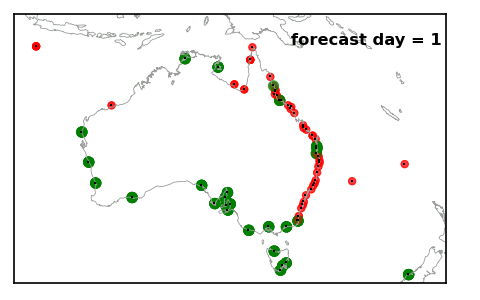
\includegraphics[width=\textwidth]{plots/plot_map_rms_score_day_1.png}
    \end{subfigure}
    \begin{subfigure}[b]{0.45\textwidth}
        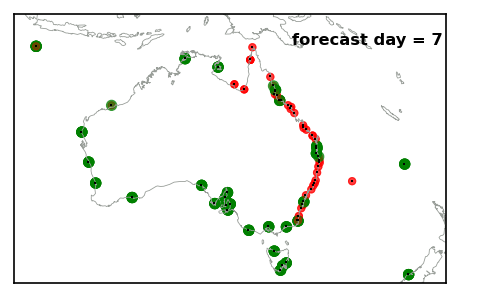
\includegraphics[width=\textwidth]{plots/plot_map_rms_score_day_7.png}
    \end{subfigure}
    \label{fig:rmsgain_b}
    \caption{ rms gain over persistance}
\end{figure}   


\begin{figure}[H]
\centering
    %------ 1
    \begin{subfigure}[a]{0.29\textwidth}
        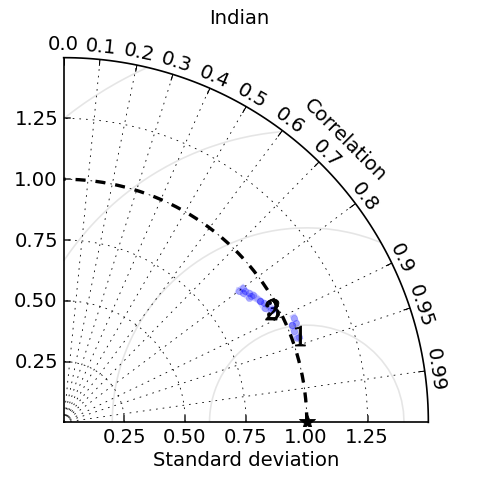
\includegraphics[width=\textwidth]{plots/taylor_diag_res_Indian.png}
    \end{subfigure}
    \begin{subfigure}[a]{0.29\textwidth}
        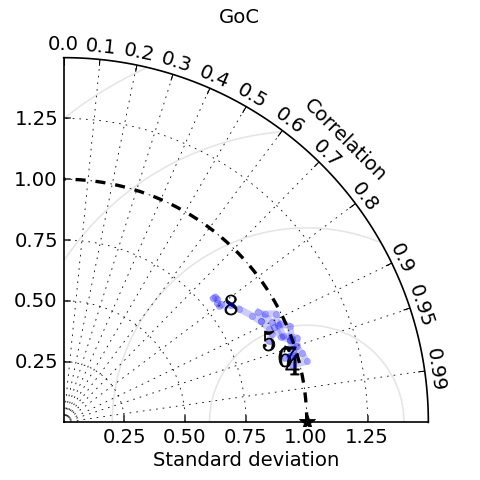
\includegraphics[width=\textwidth]{plots/taylor_diag_res_GoC.png}
    \end{subfigure}
    \begin{subfigure}[a]{0.29\textwidth}
        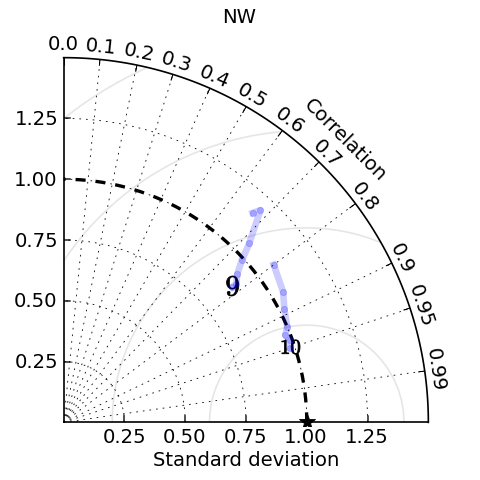
\includegraphics[width=\textwidth]{plots/taylor_diag_res_NW.png}
    \end{subfigure}
    %-------2
    \begin{subfigure}[a]{0.29\textwidth}
        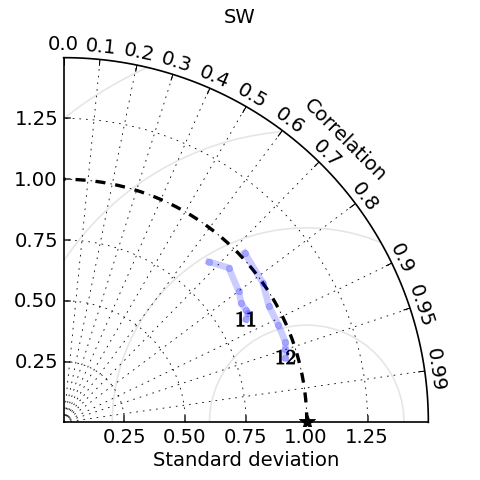
\includegraphics[width=\textwidth]{plots/taylor_diag_res_SW.png}
    \end{subfigure}
    \begin{subfigure}[a]{0.29\textwidth}
        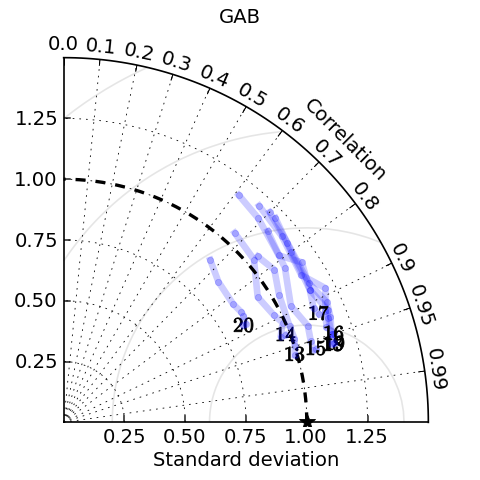
\includegraphics[width=\textwidth]{plots/taylor_diag_res_GAB.png}
    \end{subfigure}
    \begin{subfigure}[a]{0.29\textwidth}
        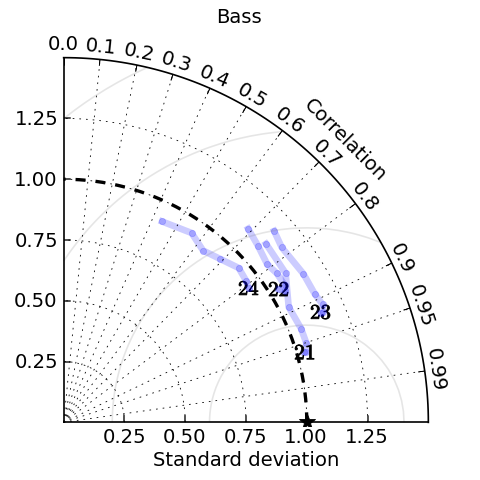
\includegraphics[width=\textwidth]{plots/taylor_diag_res_Bass.png}
    \end{subfigure}
    %-------3
    \begin{subfigure}[a]{0.29\textwidth}
        \includegraphics[width=\textwidth]{plots/taylor_diag_res_Tas.png}
    \end{subfigure}
    \begin{subfigure}[a]{0.29\textwidth}
        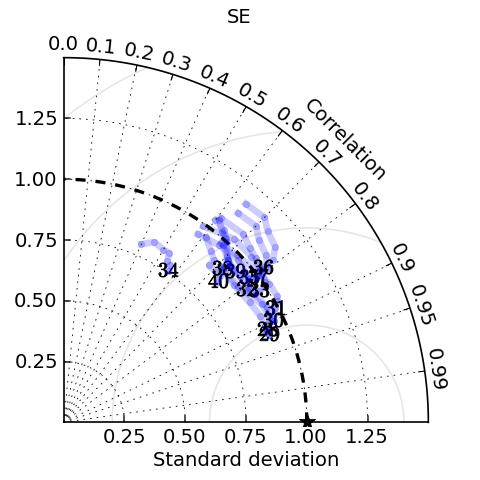
\includegraphics[width=\textwidth]{plots/taylor_diag_res_SE.png}
    \end{subfigure}
    \begin{subfigure}[a]{0.29\textwidth}
        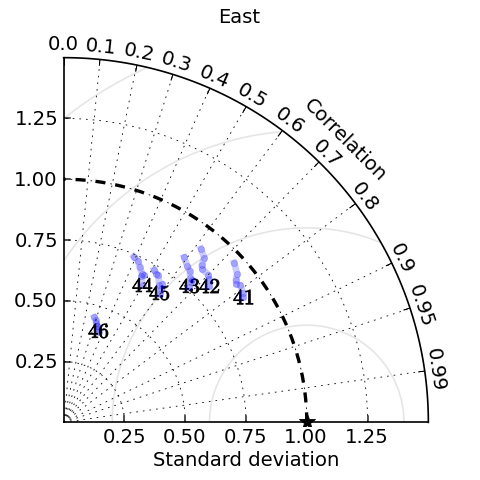
\includegraphics[width=\textwidth]{plots/taylor_diag_res_East.png}
    \end{subfigure}
    %-------4
    \begin{subfigure}[a]{0.29\textwidth}
        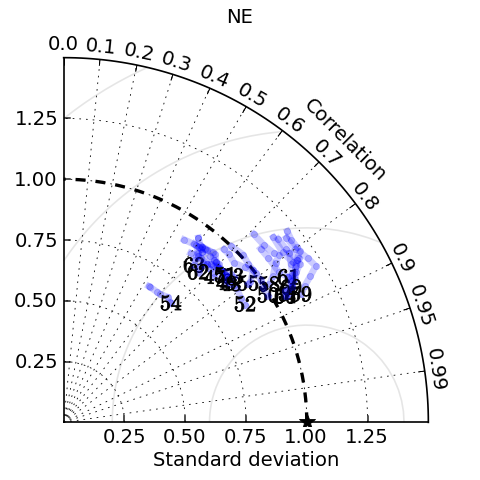
\includegraphics[width=\textwidth]{plots/taylor_diag_res_NE.png}
    \end{subfigure}
    \begin{subfigure}[a]{0.29\textwidth}
        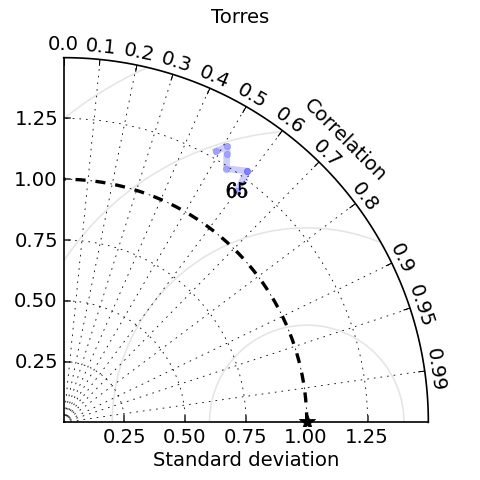
\includegraphics[width=\textwidth]{plots/taylor_diag_res_Torres.png}
    \end{subfigure}
    \begin{subfigure}[a]{0.29\textwidth}
        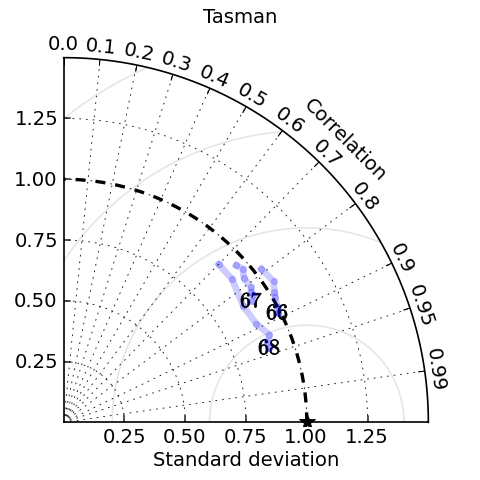
\includegraphics[width=\textwidth]{plots/taylor_diag_res_Tasman.png}
    \end{subfigure}
    %--------
    \caption{ taylor diagrams - reference non-tidal (but including long period tides) ....}
\end{figure}   



%-------------------------------------------------------------------------
\section{Bias correction component}

Multi-functional role.\\
Behaviour was not known apriori.\\
Expection of variatiobn between locations.


\begin{figure}[H]
\centering
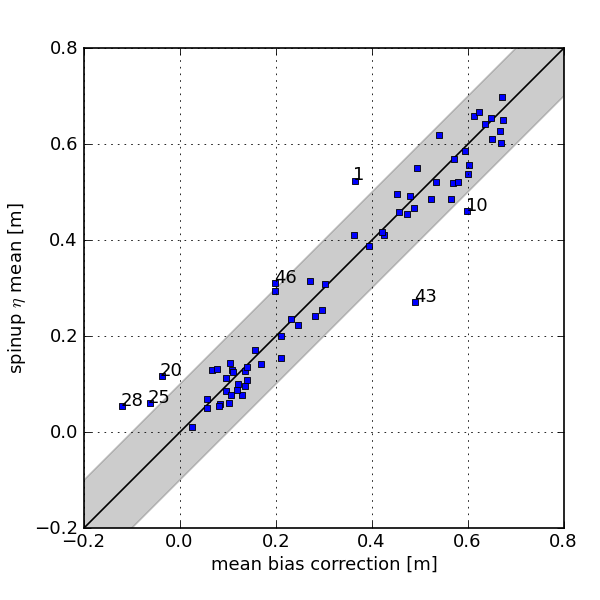
\includegraphics[width=0.3\textwidth]{plots/aggSL_bias_breakdown_plot_1.png}
\caption{ Temporal mean bias is dominated by model representation of mean dynamic topography.\\Arbtirary threshold indicated in (b)}
\end{figure}   


\begin{figure}[H]
\centering
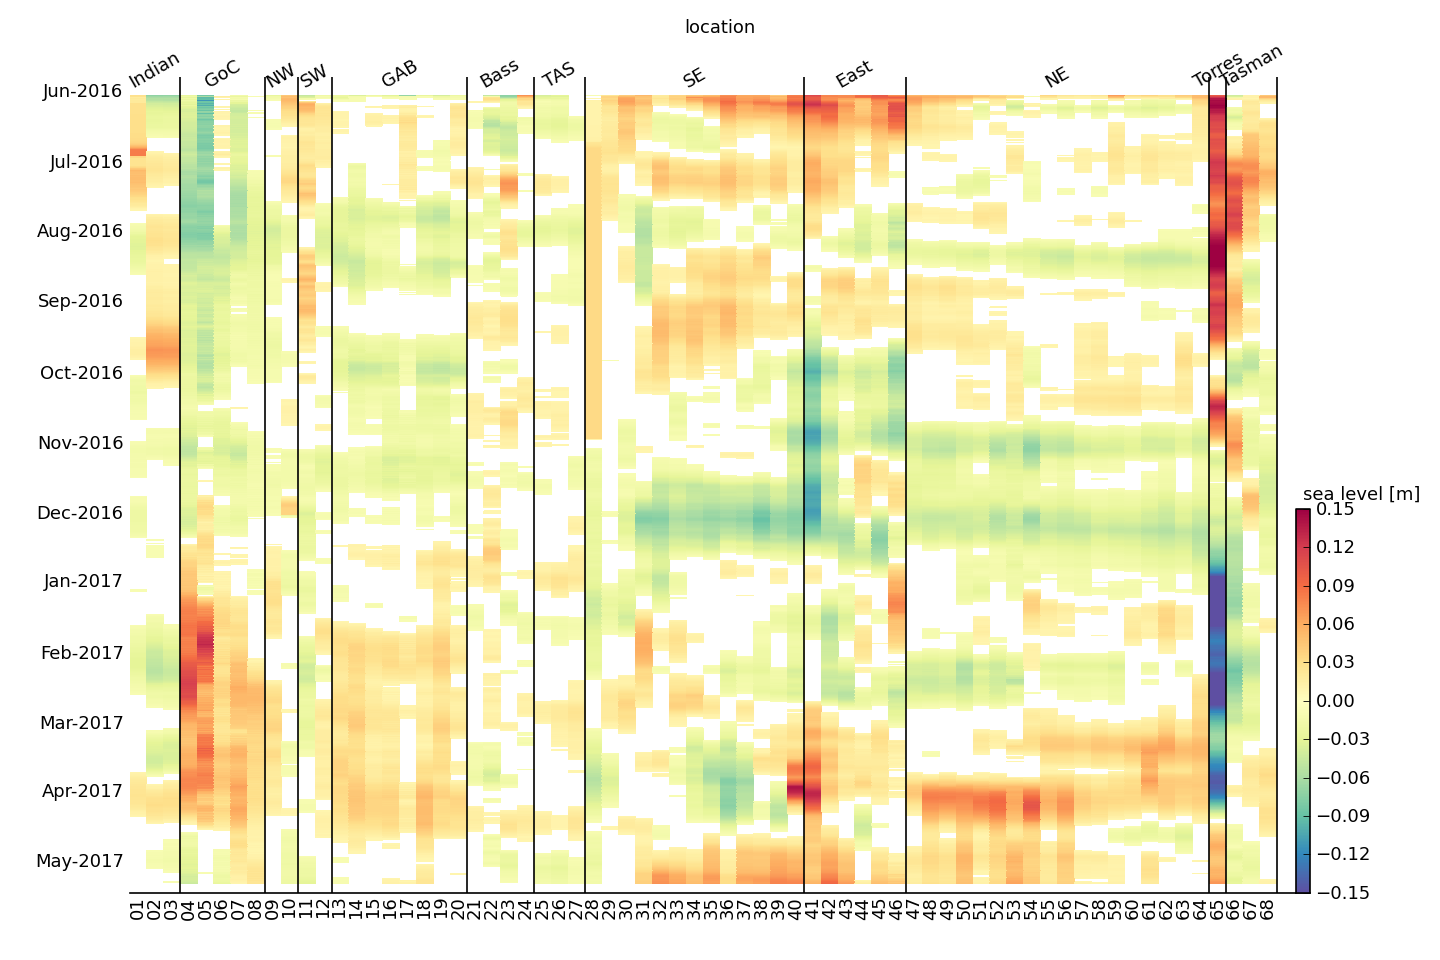
\includegraphics[width=1.1\textwidth]{plots/aggSL_bias_breakdown_plot_2.png}
\caption{ Time evolution of bias component demonstrates regional coherence }
\end{figure}  


\begin{figure}[H]
\centering
\includegraphics[width=0.8\textwidth]{plots/aggSL_corr_bias.png}
\caption{ Temporal correlation (centered by sample means).   Regional groupings apparent.  Exceptions and non-local links discussed below }
\end{figure}   



%\begin{table}[H]
%\caption{This is a table caption. Tables should be placed in the main text near to the %first time they are cited.}%
%\centering
%% \tablesize{} %% You can specify the fontsize here, e.g.  \tablesize{\footnotesize}. If commented out \small will be used.
%\begin{tabular}{ccc}
%\toprule
%\textbf{Title 1}	& \textbf{Title 2}	& \textbf{Title 3}\\
%\midrule
%entry 1		& data			& data\\
%ntry 2		& data			& data\\
%\bottomrule
%\end{tabular}
%\end{table}

%\subsection{Formatting of Mathematical Components}

%This is an example of an equation:

%\begin{equation}
%\mathbb{S}
%\end{equation}

%% If the documentclass option "submit" is chosen, please insert a blank line before and after any math environment (equation and eqnarray environments). This ensures correct linenumbering. The blank line should be removed when the documentclass option is changed to "accept" because the text following an equation should not be a new paragraph. 
%Please punctuate equations as regular text. Theorem-type envi

%%%%%%%%%%%%%%%%%%%%%%%%%%%%%%%%%%%%%%%%%%
\section{Discussion}

WIth regardt to Forecast Goodness.\\
Different aspects.


\subsection{Adequacy and value}
Are these forecasts adequate for real applications?.\\
Regional variations in skill and timescales\\
Baseline of performance.\\
Stress importance of direct evaluation against real time obs\\

\subsection{Spatial interpolation}
Can useful information be expected between observation sites??


\subsection{Explaining poor performance locations}
What is wrong with East Coast?\\
....any generic rules for exclusion?
Role of propagating signals\\
Role of harmonics\\
Role of NWP and coastal contamination\\

\subsection{Extensions and improvements to configuration}
Basic concept flexible\\
Addition of new or more inputs: eg wave setup, surge models\\
Station metadata - datums etc\\
Lagged ensemble and error estimates \\



%Authors should discuss the results and how they can be interpreted in perspective of previous studies and of the working hypotheses. The findings and their implications should be discussed in the broadest context possible. Future research directions may also be highlighted.

%%%%%%%%%%%%%%%%%%%%%%%%%%%%%%%%%%%%%%%%%%
%\section{Materials and Methods}

%Materials and Methods should be described with sufficient details to allow others to %replicate and build on published results. Please note that publication of your manuscript implicates that you must make all materials, data, computer code, and protocols associated with the publication available to readers. Please disclose at the submission stage any restrictions on the availability of materials or information. New methods and protocols should be described in detail while well-established methods can be briefly described and appropriately cited.

%Research manuscripts reporting large datasets that are deposited in a publicly available database should specify where the data have been deposited and provide the relevant accession numbers. If the accession numbers have not yet been obtained at the time of submission, please state that they will be provided during review. They must be provided prior to publication.


%%%%%%%%%%%%%%%%%%%%%%%%%%%%%%%%%%%%%%%%%%
%\section{Conclusions}

%This section is not mandatory, but can be added to the manuscript if the discussion is unusually long or complex.

%%%%%%%%%%%%%%%%%%%%%%%%%%%%%%%%%%%%%%%%%%
\vspace{6pt} 

%%%%%%%%%%%%%%%%%%%%%%%%%%%%%%%%%%%%%%%%%%
%% optional
\supplementary{The following are available online at www.mdpi.com/link,
DATA? and or FIGURES??}% Figure S1: title, Table S1: title, Video S1: title.}

%%%%%%%%%%%%%%%%%%%%%%%%%%%%%%%%%%%%%%%%%%
\acknowledgments{}
%All sources of funding of the study should be disclosed. Please clearly indicate grants that you have received in support of your research work. Clearly state if you received funds for covering the costs to publish in open access.}

%%%%%%%%%%%%%%%%%%%%%%%%%%%%%%%%%%%%%%%%%%
\authorcontributions{ TBD }
%For research articles with several authors, a short paragraph specifying their individual contributions must be provided. The following statements should be used ``X.X. and Y.Y. conceived and designed the experiments; X.X. performed the experiments; X.X. and Y.Y. analyzed the data; W.W. contributed reagents/materials/analysis tools; Y.Y. wrote the paper.'' Authorship must be limited to those who have contributed substantially to the work reported.}

%%%%%%%%%%%%%%%%%%%%%%%%%%%%%%%%%%%%%%%%%%
%\conflictsofinterest{Declare conflicts of interest or state ``The authors declare no conflict of interest.'' Authors must identify and declare any personal circumstances or interest that may be perceived as inappropriately influencing the representation or interpretation of reported research results. Any role of the funding sponsors in the design of the study; in the collection, analyses or interpretation of data; in the writing of the manuscript, or in the decision to publish the results must be declared in this section. If there is no role, please state ``The founding sponsors had no role in the design of the study; in the collection, analyses, or interpretation of data; in the writing of the manuscript, and in the decision to publish the results''.} 

%%%%%%%%%%%%%%%%%%%%%%%%%%%%%%%%%%%%%%%%%%
%% optional
\abbreviations{The following abbreviations are used in this manuscript:\\

\noindent 
\begin{tabular}{@{}ll}
NWP & Numerical Weather Prediction\\
BoM & Bureau of Meteorology\\
SLA & sea level anomaly \\
LIB & local inverse barometer\\

\end{tabular}}

%%%%%%%%%%%%%%%%%%%%%%%%%%%%%%%%%%%%%%%%%%
%% optional
%\appendixtitles{no} %Leave argument "no" if all appendix headings stay EMPTY (then no dot is printed after "Appendix A"). If the appendix sections contain a heading then change the argument to "yes".
%\appendixsections{multiple} %Leave argument "multiple" if there are multiple sections. Then a counter is printed ("Appendix A"). If there is only one appendix section then change the argument to "one" and no counter is printed ("Appendix").
%\appendix
%\section{}
%\subsection{}
%The appendix is an optional section that can contain details and data supplemental to the main text. For example, explanations of experimental details that would disrupt the flow of the main text, but nonetheless remain crucial to understanding and reproducing the research shown; figures of replicates for experiments of which representative data is shown in the main text can be added here if brief, or as Supplementary data. Mathematical proofs of results not central to the paper can be added as an appendix.

%\section{}
%All appendix sections must be cited in the main text. In the appendixes, Figures, Tables, etc. should be labeled starting with `A', e.g., Figure A1, Figure A2, etc. 

%%%%%%%%%%%%%%%%%%%%%%%%%%%%%%%%%%%%%%%%%%
% Citations and References in Supplementary files are permitted provided that they also appear in the reference list here. 

%=====================================
% References, variant A: internal bibliography
%=====================================
%\begin{thebibliography}{999}
%\bibliography{JMSE_refs}
\bibliography{references}
%
% Reference 2
%\bibitem[Author (year)]{ref-book}
%Lastname, F.F.; Author, T. The title of the cited contribution. In {\em The Book Title}; Editor, F., Meditor, A., Eds.; Publishing House: City, Country, 2007; pp. 32-58.
%\end{thebibliography}

% The following MDPI journals use author-date citation: Arts, Econometrics, Economies, Genealogy, Humanities, IJFS, JRFM, Laws, Religions, Risks, Social Sciences. For those journals, please follow the formatting guidelines on http://www.mdpi.com/authors/references

%=====================================
% References, variant B: external bibliography
%=====================================
%\externalbibliography{yes}
%\bibliography{your_external_BibTeX_file}

%%%%%%%%%%%%%%%%%%%%%%%%%%%%%%%%%%%%%%%%%%
%% optional
% \sampleavailability{Samples of the compounds ...... are available from the authors.}

%%%%%%%%%%%%%%%%%%%%%%%%%%%%%%%%%%%%%%%%%%
\end{document}

